\documentclass[11pt,twocolumn,oneside,openany,headings=optiontotoc,11pt,numbers=noenddot]{article}

\usepackage[a4paper]{geometry}
\usepackage[utf8]{inputenc}
\usepackage[T1]{fontenc}
\usepackage{lmodern}
\usepackage[ngerman]{babel}
\usepackage{ngerman}

\usepackage[onehalfspacing]{setspace}

\usepackage{fancyhdr}
\usepackage{fancybox}

\usepackage{rotating}
\usepackage{varwidth}

%Struktogramme
\usepackage[german,curves]{struktex}

\usepackage{pdflscape}
\usepackage{changepage}
\usepackage{graphicx}
\usepackage[bottom]{footmisc}
\usepackage{transparent}
\usepackage{graphbox}
\graphicspath{
	{Pics/PDFs/}
	{Pics/JPGs/}
	{Pics/PNGs/}
}
\usepackage{caption}
\usepackage{wrapfig}
\usepackage{marginnote}
\usepackage{tabularx}
\usepackage{dashrule}
\usepackage{soulutf8}
\usepackage{hhline}
%arydshln suppresses vertical lines in table
%\usepackage{arydshln}
\usepackage{multirow}
\usepackage{enumerate}
\usepackage[hidelinks]{hyperref}
\usepackage{listings}

\usepackage[table]{xcolor}
\usepackage{array}
\usepackage{enumitem,amssymb,amsmath}
\usepackage{interval}
\usepackage{cancel}
\usepackage{stmaryrd}
\usepackage{wasysym}
\usepackage{polynom}
\usepackage{diagbox}
\usepackage{dashrule}
\usepackage{framed}
\usepackage{mdframed}
\usepackage{karnaugh-map}
\usepackage{pdfpages}

\usepackage{blindtext}

\usepackage{eso-pic}

\usepackage{amssymb}
\usepackage{eurosym}

\usepackage[pages=some]{background}
\pagestyle{headings}
\renewcommand{\headrulewidth}{0.2pt}
\renewcommand{\footrulewidth}{0.2pt}
\newcommand*{\underdownarrow}[2]{\ensuremath{\underset{\overset{\Big\downarrow}{#2}}{#1}}}
\setlength{\fboxsep}{5pt}
\newcommand{\explainBelow}[3]{\underbrace{#1}_{\parbox{\widthof{#3}}{\footnotesize\raggedright #2}}}
\newcommand{\explainAbove}[3]{\overbrace{#1}^{\parbox{\widthof{#3}}{\footnotesize\raggedright #2}}}
\newcommand\footnoteref[1]{\protected@xdef\@thefnmark{\ref{#1}}\@footnotemark}


% Codestyle defined
\definecolor{codegreen}{rgb}{0,0.6,0}
\definecolor{codegray}{rgb}{0.5,0.5,0.5}
\definecolor{codepurple}{rgb}{0.58,0,0.82}
\definecolor{backcolour}{rgb}{0.95,0.95,0.92}
\definecolor{deepgreen}{rgb}{0,0.5,0}
\definecolor{darkblue}{rgb}{0,0,0.65}
\definecolor{mauve}{rgb}{0.40, 0.19,0.28}
\colorlet{exceptioncolour}{yellow!50!red}
\colorlet{commandcolour}{blue!60!black}
\colorlet{numpycolour}{blue!60!green}
\colorlet{specmethodcolour}{violet}

%Neue Spaltendefinition
\newcolumntype{L}[1]{>{\raggedright\let\newline\\\arraybackslash\hspace{0pt}}m{#1}}
\newcolumntype{M}{>{\centering\arraybackslash}X}
\newcommand{\cmnt}[1]{\ignorespaces}
%Textausrichtung ändern
\newcommand\tabrotate[1]{\rotatebox{90}{\raggedright#1\hspace{\tabcolsep}}}

%Intervall-Konfig
\intervalconfig {
	soft open fences
}

%Bash
\lstdefinestyle{BashInputStyle}{
	language=bash,
	basicstyle=\small\sffamily,
	backgroundcolor=\color{backcolour},
	columns=fullflexible,
	backgroundcolor=\color{backcolour},
	breaklines=true,
}
%Java
\lstdefinestyle{JavaInputStyle}{
	language=Java,
	backgroundcolor=\color{backcolour},
	aboveskip=1mm,
	belowskip=1mm,
	showstringspaces=false,
	columns=flexible,
	basicstyle={\footnotesize\ttfamily},
	numberstyle={\tiny},
	numbers=none,
	keywordstyle=\color{purple},,
	commentstyle=\color{deepgreen},
	stringstyle=\color{blue},
	emph={out},
	emphstyle=\color{darkblue},
	emph={[2]rand},
	emphstyle=[2]\color{specmethodcolour},
	breaklines=true,
	breakatwhitespace=true,
	tabsize=2,
}
%Python
\lstdefinestyle{PythonInputStyle}{
	language=Python,
	alsoletter={1234567890},
	aboveskip=1ex,
	basicstyle=\footnotesize,
	breaklines=true,
	breakatwhitespace= true,
	backgroundcolor=\color{backcolour},
	commentstyle=\color{red},
	otherkeywords={\ , \}, \{, \&,\|},
	emph={and,break,class,continue,def,yield,del,elif,else,%
		except,exec,finally,for,from,global,if,import,in,%
		lambda,not,or,pass,print,raise,return,try,while,assert},
	emphstyle=\color{exceptioncolour},
	emph={[2]True,False,None,min},
	emphstyle=[2]\color{specmethodcolour},
	emph={[3]object,type,isinstance,copy,deepcopy,zip,enumerate,reversed,list,len,dict,tuple,xrange,append,execfile,real,imag,reduce,str,repr},
	emphstyle=[3]\color{commandcolour},
	emph={[4]ode, fsolve, sqrt, exp, sin, cos, arccos, pi,  array, norm, solve, dot, arange, , isscalar, max, sum, flatten, shape, reshape, find, any, all, abs, plot, linspace, legend, quad, polyval,polyfit, hstack, concatenate,vstack,column_stack,empty,zeros,ones,rand,vander,grid,pcolor,eig,eigs,eigvals,svd,qr,tan,det,logspace,roll,mean,cumsum,cumprod,diff,vectorize,lstsq,cla,eye,xlabel,ylabel,squeeze},
	emphstyle=[4]\color{numpycolour},
	emph={[5]__init__,__add__,__mul__,__div__,__sub__,__call__,__getitem__,__setitem__,__eq__,__ne__,__nonzero__,__rmul__,__radd__,__repr__,__str__,__get__,__truediv__,__pow__,__name__,__future__,__all__},
	emphstyle=[5]\color{specmethodcolour},
	emph={[6]assert,range,yield},
	emphstyle=[6]\color{specmethodcolour}\bfseries,
	emph={[7]Exception,NameError,IndexError,SyntaxError,TypeError,ValueError,OverflowError,ZeroDivisionError,KeyboardInterrupt},
	emphstyle=[7]\color{specmethodcolour}\bfseries,
	emph={[8]taster,send,sendMail,capture,check,noMsg,go,move,switch,humTem,ventilate,buzz},
	emphstyle=[8]\color{blue},
	keywordstyle=\color{blue}\bfseries,
	rulecolor=\color{black!40},
	showstringspaces=false,
	stringstyle=\color{deepgreen}
}

\lstset{literate=%
	{Ö}{{\"O}}1
	{Ä}{{\"A}}1
	{Ü}{{\"U}}1
	{ß}{{\ss}}1
	{ü}{{\"u}}1
	{ä}{{\"a}}1
	{ö}{{\"o}}1
}

% Neue Klassenarbeits-Umgebung
\newenvironment{worksheet}[3]
% Begin-Bereich
{
	\newpage
	\sffamily
	\setcounter{page}{1}
	\ClearShipoutPicture
	\AddToShipoutPicture{
		\put(55,761){{
				\mbox{\parbox{385\unitlength}{\tiny \color{codegray}BBS I Mainz, #1 \newline #2
						\newline #3
					}
				}
			}
		}
		\put(455,761){{
				\mbox{\hspace{0.3cm}
\includegraphics[width=0.2\textwidth]{../../logo.pdf}}
			}
		}
	}
}
% End-Bereich
{
	\clearpage
	\ClearShipoutPicture
}

\setlength{\columnsep}{3em}
\setlength{\columnseprule}{0.5pt}

\geometry{left=2.00cm,right=2.00cm,top=3.00cm,bottom=1.00cm,includeheadfoot}
\pagenumbering{arabic}
\pagestyle{plain}

\begin{document}
	\begin{worksheet}{BS FI}{1. Lehrjahr, LF 4 - Einfache IT-Systeme}{Digitaltechnik}
		\setcounter{section}{6}
		\section{Schaltungen analysieren}
		Bisher haben wir aus der geforderten Funktionalität eine Funktionstabelle und daraus eine logische Funktion aufgestellt. Mit dieser Funktion haben wir dann die Schaltung in einer Simulationssoftware\footnote{LogicSim} realisiert und getestet.\\
		\par\noindent
		\texttt{Was aber, wenn wir die Schaltung erhalten und deren Funktionalität beschreiben sollen?}\\
		\subsection*{Funktionsweisen einer Schaltung beschreiben}
		Wir nutzen die folgende Schaltung beispielhaft zur Verdeutlichung des Vorgehens.\\
		\par\noindent
		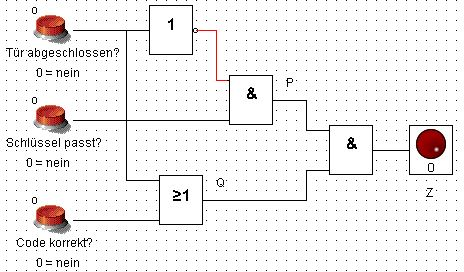
\includegraphics[width=0.48\textwidth]{../99_Bilder/schAna.jpg}\\
		\par\noindent
		(I) Wir beginnen mit der \textbf{Funktionstabelle}.\\
		In diese Übertragen wir die \textbf{Ein- und Ausgangsvariablen}.\\
		Eingangsvarablen: \(Tür = T, Schlüssel = S, Code = C\)\\
		Ausgangsvariable: \(LED = L\)
		\begin{framed}
			\noindent
			\footnotesize{Wenn nötig, kann die Schaltung auch in kleinere Abschnitte (im Beispiel \(P\) und \(Q\)) unterteilt werden.\\
			Diese Spalten \(P\) und \(Q\) dienen lediglich als \textbf{Zwischenschritt} um die Gesamtsituation \(Z\) korrekt auszufüllen.\\
			Sie \underline{müssen nicht} bei jeder Analyse angegeben werden.}
		\end{framed}
		\begin{tabularx}{0.48\textwidth}{|M|M|M||M|M||M|}
			\hline
			\rowcolor{codegray!10} \(A\) & \(B\) & \(C\) & \(P\) & \(Q\) & \(LED\) \\
			\rowcolor{codegray!15} & & & \(\overline{A} \wedge{} B\) & \(A \vee{} C\) & \(P \wedge{} Q\)\\
			\hline
			0 & 0 & 0 & & &\\
			\hline
			0 & 0 & 1 & & &\\
			\hline
			0 & 1 & 0 & & &\\
			\hline
			0 & 1 & 1 & & &\\
			\hline
			1 & 0 & 0 & & &\\
			\hline
			1 & 0 & 1 & & &\\
			\hline
			1 & 1 & 0 & & &\\
			\hline
			1 & 1 & 1 & & &\\
			\hline
		\end{tabularx}\\
		\par\noindent
		(II) Im Anschluss betrachten wir die einzelnen (oder die gesamte ) Situationen \(P\) und \(Q\).\\
		Wir befüllen die Spalten der einzelnen Situationen (\(P = \overline{A}\wedge{}B\) bzw. \(Q = A \vee{} C\)) unter Berücksichtigung der Variablenzustände.\\
		\par\noindent
		\begin{tabularx}{0.48\textwidth}{|M|M|M||M|M||M|}
			\hline
			\rowcolor{codegray!10} \(A\) & \(B\) & \(C\) & \(P\) & \(Q\) & \(LED\) \\
			\rowcolor{codegray!15} & & & \(\overline{A} \wedge{} B\) & \(A \vee{} C\) & \(P \wedge{} Q\)\\
			\hline
			0 & 0 & 0 & 0 & 0 &\\
			\hline
			0 & 0 & 1 & 0 & 1 &\\
			\hline
			0 & 1 & 0 & 1 & 0 &\\
			\hline
			0 & 1 & 1 & 1 & 1 &\\
			\hline
			1 & 0 & 0 & 0 & 1 &\\
			\hline
			1 & 0 & 1 & 0 & 1 &\\
			\hline
			1 & 1 & 0 & 0 & 1 &\\
			\hline
			1 & 1 & 1 & 0 & 1 &\\
			\hline
		\end{tabularx}\\
		\par\noindent
		(III) Mit Hilfe der Einzelsituationen \(P\) und \(Q\) betrachten wir nun die Gesamtsituation \(Z = P \wedge{} Q\) und füllen diese Spalte entsprechend.\\
		\par\noindent
		\begin{tabularx}{0.48\textwidth}{|M|M|M||M|M||M|}
			\hline
			\rowcolor{codegray!10} \(Tür\) & \(B\) & \(C\) & \(P\) & \(Q\) & \(LED\) \\
			\rowcolor{codegray!15} & & & \(\overline{A} \wedge{} B\) & \(A \vee{} C\) & \(P \wedge{} Q\)\\
			\hline
			0 & 0 & 0 & 0 & 0 & 0\\
			\hline
			0 & 0 & 1 & 0 & 1 & 0\\
			\hline
			0 & 1 & 0 & 1 & 0 & 0\\
			\hline
			\rowcolor{green!10} 0 & 1 & 1 & 1 & 1 & 1\\
			\hline
			1 & 0 & 0 & 0 & 1 & 0\\
			\hline
			1 & 0 & 1 & 0 & 1 & 0\\
			\hline
			1 & 1 & 0 & 0 & 1 & 0\\
			\hline
			1 & 1 & 1 & 0 & 1 & 0\\
			\hline
		\end{tabularx}\\
		\par\noindent
		(IV) Für die Beschreibung der Schaltung sind nun ausschließlich die Zeilen relevant, bei denen die Gesamtsituation \(Z = 1\) ist.\\
		Für diese betrachten wir die Zustände der Eingangsvariablen und formulieren unter Zuhilfenahme der Situation die Funktionalität.\\
		\par\noindent
		\setlength{\leftskip}{0.5cm}
		\textit{\textbf{Die LED leuchtet auf, wenn die Tür nicht abgeschlossen ist, der Schlüssel passt und der eingegebene Code korrekt ist.}}\\
		\par\noindent
		\setlength{\leftskip}{0cm}
		\texttt{\underline{Die Vorgehensweise im Überblick}}
		\begin{itemize}
			\item[(I)] Ein- und Ausgangsvariablen bestimmen\\
			Funktionstabelle mit Variablen aufstellen
			\item[(II)] Teilsituationen in Funktionstabelle übernehmen und entsprechende Ausgänge eintragen
			\item[(III)] Gesamtsituation in Tabelle angeben unter Berücksichtigung der Einzelsituationen füllen
			\item[(IV)] Betrachte ausschließlich die Zeilen der Funktionstabelle, in denen die Gesamtsituation den Zustand \(1\) hat.\\
			Nutze die Eingangsvariablen zur Beschreibung der Funktionalität.
		\end{itemize}
	\end{worksheet}
\end{document}